\hypertarget{development-of-reactive-machine-models}{%
\section{Development of Reactive Machine
Models}\label{development-of-reactive-machine-models}}

Domain-Oriented Process-Control

\begin{itemize}
\tightlist
\item
  Domain-Oriented: Correspondence with technical-processes
\item
  Process-Control: Control of the technical-processes
\end{itemize}

\hypertarget{correspondence}{%
\subsection{Correspondence}\label{correspondence}}

\begin{itemize}
\tightlist
\item
  Static Correspondence

  \begin{itemize}
  \tightlist
  \item
    Technical-process \textless{}-\textgreater{} reactive-object
    (boundary-object)
  \end{itemize}
\item
  Dynamic Correspondence

  \begin{itemize}
  \tightlist
  \item
    Boundary-object handles exactly the same event-sequences that are
    generated by the correspondingtechnical-Process
  \end{itemize}
\end{itemize}

\hypertarget{static-correspondence}{%
\subsubsection{Static Correspondence}\label{static-correspondence}}

\begin{itemize}
\tightlist
\item
  Parallel technical-processes generate parallel event sequences
\item
  These are received from the embedded-system as a sequential stream of
  events
\item
  This stream is disentangled and the messages are forwarded to their
  proper receiver reactive-objects(boundary-objects)
\item
  Boundary-objects communicate virtually with technical-processes
\end{itemize}

\begin{figure}[H]
\centering
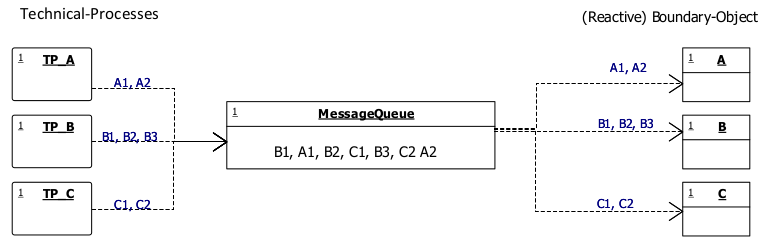
\includegraphics[width=1\textwidth]{figures/staticCorrespondence.png}
\caption{Static Correspondence}
\end{figure}

\clearpage
\hypertarget{dynamic-correspondence}{%
\subsubsection{Dynamic Correspondence}\label{dynamic-correspondence}}

\begin{itemize}
\tightlist
\item
  A technical-process may be considered as a state-machine
\item
  The technical-processes and the embedded-system communicate via
  virtual interaction
\item
  Dynamic correspondence means:

  \begin{itemize}
  \tightlist
  \item
    The boundary-object has to expect the event sequences generated by
    the technical-process, and must be able to handle them
  \item
    The finite state-machine of the boundary-object must be based on the
    behaviour of the technical-process
  \item
    Context-model
  \end{itemize}
\end{itemize}

\textbf{Context-Model Example 1}
\begin{figure}[H]
\centering
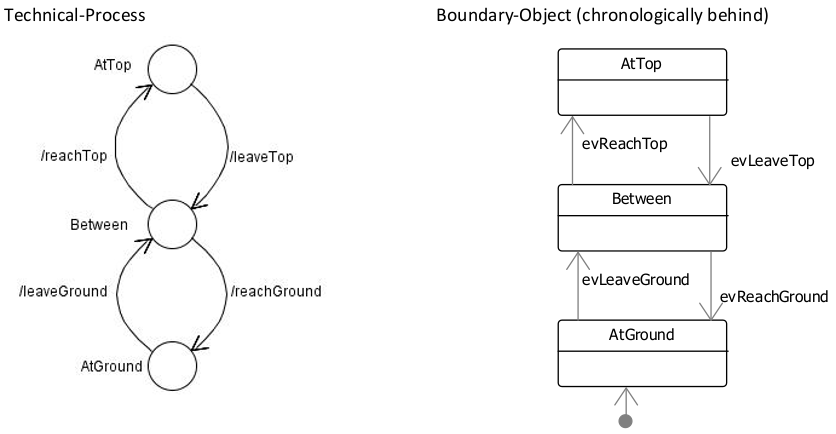
\includegraphics[width=0.9\textwidth]{figures/dynamicCorrespondence.png}
\caption{Context-Model Example 1}
\end{figure}

\clearpage
\textbf{Context-Model Example 2}
\begin{figure}[H]
\centering
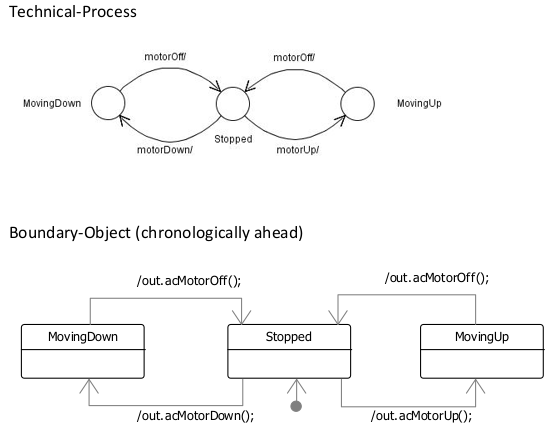
\includegraphics[width=0.8\textwidth]{figures/dynamicCorrespondence2.png}
\caption{Context-Model Example 2}
\end{figure}

\begin{itemize}
\tightlist
\item
  In Example 1 and Example 2, we are only observing
\item
  While observing, we are chronically behind the technical process
\item
  In Example 3 and Example 4, we are observing and controlling
\item
  When observing and controlling at the same time, we are sometimes
  behind and sometimes before the technical process
\item
  In the sequence diagram, you see that the external process sometimes
  is before and sometimes is behind the boundary object
\end{itemize}

\clearpage
\textbf{Context-Model Example 3}
\begin{figure}[H]
\centering
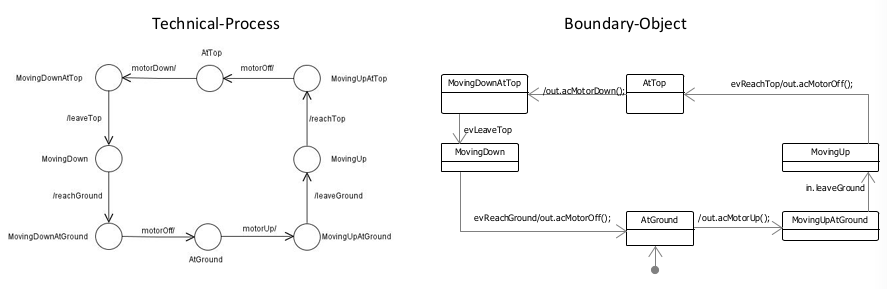
\includegraphics[width=0.8\textwidth]{figures/dynamicCorrespondence3.png}
\caption{Context-Model Example 3}
\end{figure}

\begin{figure}[H]
\centering
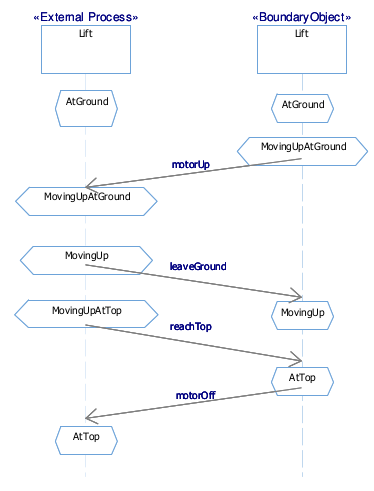
\includegraphics[width=0.7\textwidth]{figures/sequenceToDynamicCorrespondenceExample.png}
\caption{Dynamic Correspondence 3 Sequence}
\end{figure}

\clearpage
\textbf{Context-Model Example 4}
\begin{figure}[H]
\centering
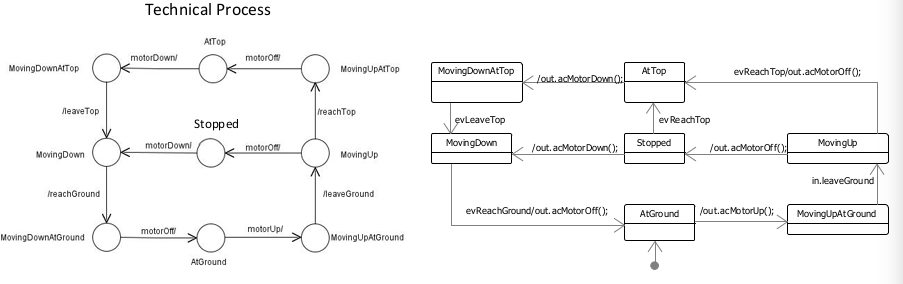
\includegraphics[width=1\textwidth]{figures/dynamicCorrespondence4.png}
\caption{Context-Model Example 4}
\end{figure}

\hypertarget{development-process}{%
\subsection{Development Process}\label{development-process}}

\begin{itemize}
\tightlist
\item
  Define events and actions
\item
  Context-model: Boundary-objects
\item
  Control-Functions: Cooperation of boundary-objects and other
  reactive-objects
\end{itemize}

\hypertarget{step-1---events-and-actions}{%
\subsubsection{Step 1 - Events and
Actions}\label{step-1---events-and-actions}}

\begin{figure}[H]
\centering
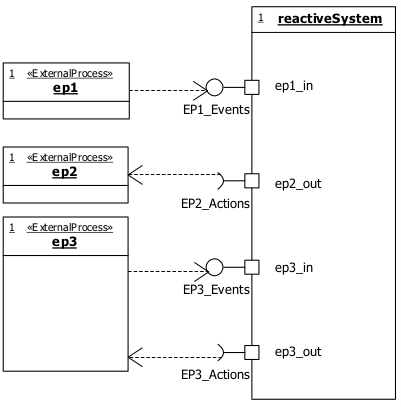
\includegraphics[width=0.4\textwidth]{figures/step1ReactiveMachineModelsDevelopment.png}
\caption{Step 1}
\end{figure}

\begin{itemize}
\tightlist
\item
  For each technical-process, define event- and action-ports, i.e.
  (In-Ports and Out-Ports)
\item
  For each port define the set of event- or action messages
  -\textgreater{} interfaces
\item
  The reactive-system consists of one or more reactive-clusters
\end{itemize}

\hypertarget{step-2---context-model}{%
\subsubsection{Step 2 - Context-Model}\label{step-2---context-model}}

\begin{figure}[H]
\centering
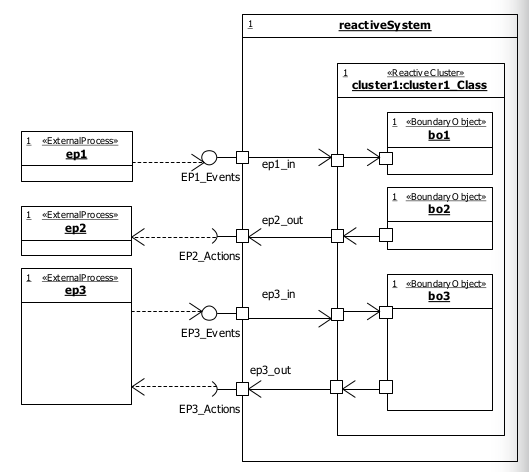
\includegraphics[width=0.5\textwidth]{figures/step2ReactiveMachineModelsDevelopment.png}
\caption{Step 2}
\end{figure}

\begin{itemize}
\tightlist
\item
  The context-model consists of a set of boundary-objects
\item
  Boundary-objects

  \begin{itemize}
  \tightlist
  \item
    Are reactive-objects
  \item
    Virtually connected to the technical processes
  \item
    The state-machines of the boundary objects define the valid
    sequences of event- and action-Messages
  \end{itemize}
\end{itemize}

\hypertarget{step-3---control-functions}{%
\subsubsection{Step 3 -
Control-Functions}\label{step-3---control-functions}}

\begin{figure}[H]
\centering
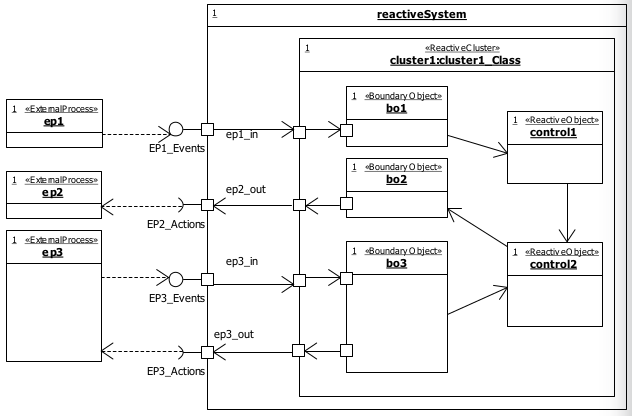
\includegraphics[width=0.73\textwidth]{figures/step3ReactiveMachineModelsDevelopment.png}
\caption{Step 3}
\end{figure}

\begin{itemize}
\tightlist
\item
  Perhaps completed by control-objects
\item
  Control-Objects

  \begin{itemize}
  \tightlist
  \item
    Are reactive-objects
  \item
    Do not interact virtually with the technical-process
  \item
    Interact only with other reactive objects
  \item
    Are responsible for the real control functions
  \item
    Do not correspond to a technical process
  \end{itemize}
\end{itemize}

\hypertarget{context-errors}{%
\subsubsection{Context Errors}\label{context-errors}}

Context-errors arise if an event occurs that contradicts the
context-model. This could have two reasons:

\begin{enumerate}
\def\labelenumi{\arabic{enumi}.}
\tightlist
\item
  An event sequence that can occur in a correctly working system, is not
  handled by the context-model
\item
  An event that should not occur in a given state of the
  technical-process
\end{enumerate}

\hypertarget{race-conditions}{%
\subsection{Race Conditions}\label{race-conditions}}

A \textbf{Race-Condition} in an embedded-system is a situation where two
or more events can occur simultaneously.

\begin{itemize}
\tightlist
\item
  In such cases the arrival order of the corresponding event-messages is
  random
\item
  Consequence for the behaviour model: All possible sequences have to be
  taken into account
\end{itemize}

\clearpage